\documentclass[border=0.65cm,tikz]{standalone}
\usepackage[utf8]{vietnam}
\usepackage{xparse}
\usepackage{xcolor}
\definecolor{dnvang}{HTML}{D8A25E}
\definecolor{dnxanh}{HTML}{229799}
\definecolor{dnxanhdam}{HTML}{0D7C66}
\definecolor{dndo}{HTML}{BB2649}
\def\mycolor{dnvang}
\def\mauphu{dnxanh}
\def\maudam{dnxanhdam}
\def\maunhan{dndo}
\usepackage{tikz}
\usepackage{tikz-3dplot}
\usepackage{pgfplots}
\pgfplotsset{compat=1.18}
\usetikzlibrary{angles,quotes,intersections,fit}
\usetikzlibrary{calc,fadings,shadows,shadows.blur,shapes,shapes.geometric,positioning,backgrounds,decorations.pathmorphing,decorations,matrix}
\usetikzlibrary{decorations.pathmorphing}
\usepackage{amsmath}
\begin{document}
	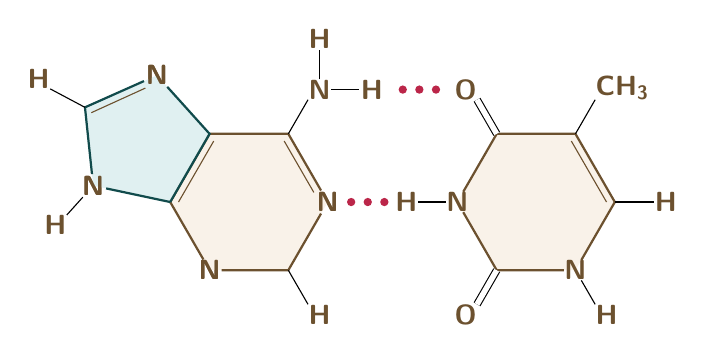
\begin{tikzpicture}[declare function={r=1;},double distance=2pt,font=\bfseries,text=\mycolor!50!black]
	%%Vẽ khung lục giác vòng 1%%
		\path[\mycolor!30](180:r) coordinate (C1)
		--++(0:r) coordinate (C2)
		--++(-60:r) coordinate (C3)
		--++(-120:r) coordinate (C4) node[inner sep=0pt,font=\sffamily\bfseries] (N1){N}
		--++(180:r) coordinate (C5)
		--++(120:r) coordinate (C6) node[inner sep=0pt,font=\sffamily\bfseries] (N2){N}
		(N1)--(C1)
		;
		\path[fill=\mycolor!20,opacity=0.7] (C1)--(C2)--(C3)--(C4)--(C5)--(C6)--cycle;
		%%%Vẽ nối đôi
		\draw[\mycolor!50!black] ($(C2)+(-120:3pt)$)--($(C3)+(180:3pt)$);
		\draw[\mycolor!50!black,thick] (C1)--(C2)--(C3)--(N1)--(C5)--(N2)--(C1);
		\path (C4) node[inner sep=0pt,font=\sffamily\bfseries]{N}
		(C6)node[inner sep=0pt,font=\sffamily\bfseries]{N}
		;
		%%%Vẽ các nhánh vòng 1
		\foreach [count=\i from 1] \s\p/\g/\a/\n in {%
			double/C1/120/south east/O,
			{}/C2/60/south west/CH$_\text{3}$,
			{}/C3/0/west/H,
			{}/N1/-60/north west/H,
			double/C5/-120/north east/O,
			{}/N2/180/east/H
			}{%
			\path [draw,\s] (\p)--++(\g:0.5cm) node [anchor=\a,inner sep=0pt,font=\sffamily\bfseries] (br-\i){\n};
		}
		%%%Vẽ khung lục giác vòng 2
		\path ($(br-6)+(180:r)$) coordinate (Goc) node[anchor=center,inner sep=0.5pt,font=\sffamily\bfseries] (N3) {N};
		
		\path[\mycolor!50!black,thick] (Goc)--++(120:r) coordinate (Ca)
		--++(180:r) coordinate (Cb)
		--++(-120:r) coordinate (Cc)
		--++(-60:r) coordinate (Cd) node[anchor=center,inner sep=0pt,font=\sffamily\bfseries] (N4) {N}
		--++(0:r) coordinate (Ce)
		;
		\path[fill=\mycolor!20,opacity=0.7] (Goc)--(Ca)--(Cb)--(Cc)--(Cd)--(Ce)--cycle;
		\path[draw=\mycolor!50!black,thick] (N3)--(Ca)--(Cb)--(Cc)--(N4)--(Ce)--(N3);
		\path (Goc) node[inner sep=0pt,font=\sffamily\bfseries]{N}
		(Cd) node[inner sep=0pt,font=\sffamily\bfseries]{N}
		;
		%%vẽ liên kết đôi
		\draw[\mycolor!50!black,shorten <=4pt] ($(Goc)+(180:3pt)$)--($(Ca)+(-120:3pt)$);
		\draw[\mycolor!50!black] ($(Cb)+(-60:3pt)$)--($(Cc)+(0:3pt)$);
		%%%Vẽ vòng 5 cạnh
		\path (Cc)--(Cb)
		--++(132:r) coordinate (B1) node[inner sep=0.5pt,font=\sffamily\bfseries](N5) {N}
		--([turn]72:r) coordinate (B2) 
		--([turn]72:r) coordinate (B3) node[inner sep=0.5pt,font=\sffamily\bfseries](N6) {N}
		--([turn]72:r) coordinate (B4)
		;
		\path[fill=\mauphu!20,opacity=0.7] (Cc)--(Cb)--(B1)--(B2)--(B3)--(B4)--cycle;
		\path[draw=\mauphu!50!black,thick] (Cc)--(Cb)--(N5)--(B2)--(N6)--(B4)--cycle;
		%%%Vẽ nối đôi
		\draw[\mycolor!50!black,shorten <=4pt] ($(B1)+(-100:3pt)$)--($(B2)+(-40:3pt)$);
		\path (B3) node[inner sep=0pt,font=\sffamily\bfseries]{N}
		(B1) node[inner sep=0pt,font=\sffamily\bfseries]{N}
		;
		%%%Vẽ các nhánh vòng 2
		\foreach [count=\i from 1] \s\p/\g/\a/\n in {%
			{}/Ca/60/south west/N,
			{}/Ce/-60/north west/H,
			{}/B2/152/south east/H,
			{}/N6/-132/north east/H
		}{%
			\path [draw,\s] (\p)--++(\g:0.5cm) node [anchor=\a,inner sep=0pt,font=\sffamily\bfseries] (nhanh-\i){\n};
		}
		%%%Vẽ nhánh phụ
		\draw (nhanh-1)--++(0:0.5) node [anchor=west,font=\sffamily\bfseries,inner sep=0.5pt] (Ha) {H};
		\draw (nhanh-1)--++(90:0.5) node [anchor=south,font=\sffamily\bfseries,inner sep=0.5pt] {H};
		%%Vẽ liên kết H
		\path (br-1)--(Ha) node[midway,sloped]{\tikz\fill[\maunhan] (0,0) circle (1.5pt) (6pt,0) circle (1.5pt)(12pt,0) circle (1.5pt);};
		\path (br-6)--(N3) node[midway,sloped]{\tikz\fill[\maunhan] (0,0) circle (1.5pt) (6pt,0) circle (1.5pt)(12pt,0) circle (1.5pt);};
	\end{tikzpicture}
\end{document}